\documentclass[a4paper]{article}
\usepackage{fontspec}
\usepackage{amsmath}
\usepackage{amssymb}


%%%%lualatex on
%\usepackage{luatextra}
%Ligatures={Contextual, Common, Historical, Rare, Discretionary}
%\setmainfont[Mapping=tex-text]{Linux Libertine O}

\usepackage{natbib}

\title{Note about WSC}
\author{Simon}
\begin{document}
\maketitle
\section{Cultural Evolution}


We run a first set of experiment where all agents interact with everyone. The only evolutionary mechanism are .Following \cite{bentley2004randomdriftandculturechange}

\subsection{One trait}

The Finite Innovation Effect (ie : $n$ variant  $| n\in\{0,\cdots,100\}$) :
\begin{figure}[h]
	\begin{center}
		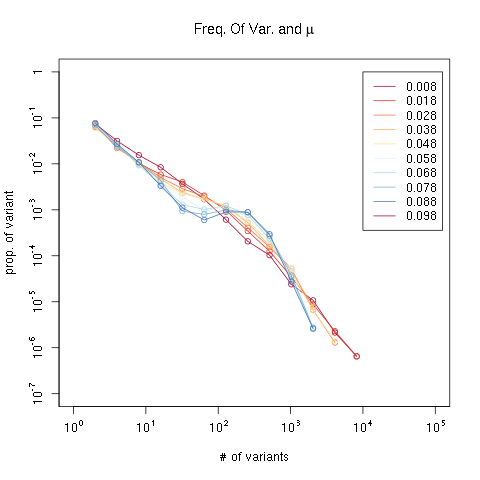
\includegraphics[width=7cm]{../../epnet-dev/analtest/allmu.png}
	\end{center}
	\caption{rand()\%100}
	\label{fig:finitEffect}
\end{figure}


With infinite innovation possibilities(ie : $n$ variant $| n\in\mathbb{A} $):
\begin{figure}[hbp]
	\begin{center}
		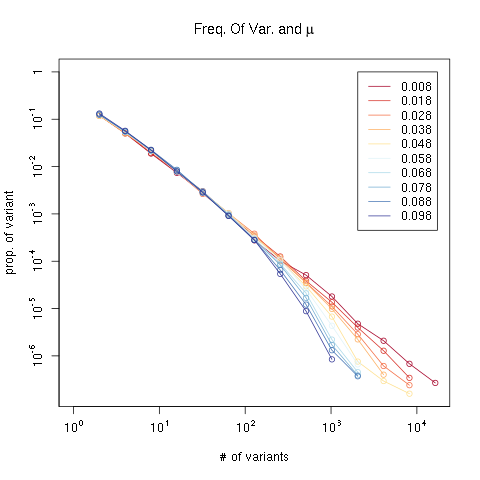
\includegraphics[width=7cm]{../../epnet-dev/analtest/allmuRandMax.png}
	\end{center}
	\caption{rand()\%RAND\_MAX}
	\label{fig:allMutation}
\end{figure}


\section{Multiple Traits (all varying on $\mathbb{N}$)}
In that case individual owns a vector of $n$ traits. One a cultural exchange occurs the whole vector is exchanged.

In the case individual carries multiples traits (ie price in our experiment), we check that it does not change the result of the algorithm in the long terms, each traits will evolve following the same curves than when juste one traits is evolving and exchange.
\begin{figure}[h]
	\begin{center}
		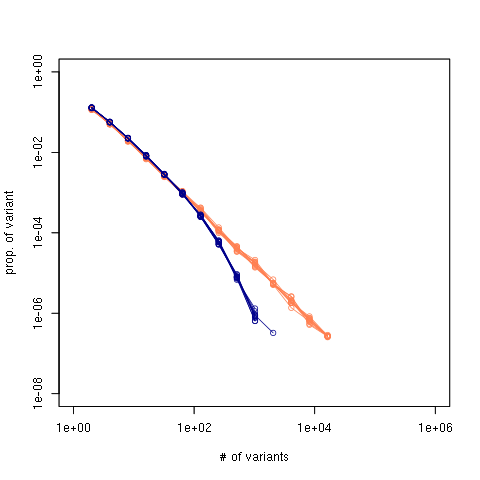
\includegraphics[width=6cm]{../../epnet-dev/analtest/10resources.png}
	\end{center}
	\caption{$\mu=\{.08,.098\}$ for 10 resources}
	\label{fig:10resources}
\end{figure}

\begin{figure}[h]
	\begin{center}
		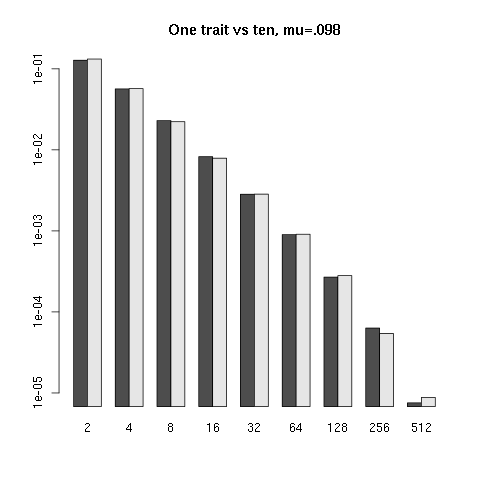
\includegraphics[width=6cm]{../../epnet-dev/analtest/OneVsTenMu098.png}
		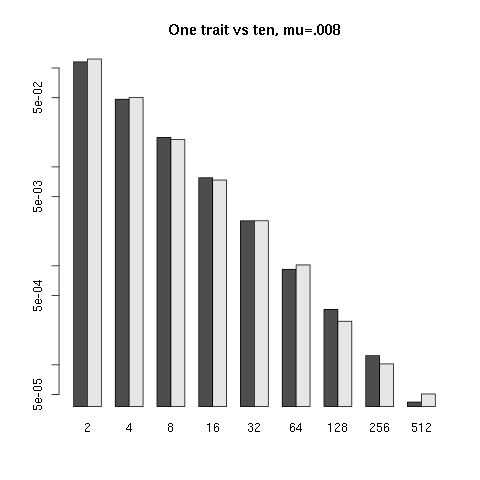
\includegraphics[width=6cm]{../../epnet-dev/analtest/OneVsTenMu008.png}
	\end{center}
	\caption{$\mu=\{.08,.098\}$ for one of the 10 resources VS one only}
	\label{fig:OneVsTen}
\end{figure}

\bibliographystyle{apalike}
\bibliography{/home/scarrign/Documents/biblio/bib/phd.bib}  
\end{document}


